\documentclass[10pt,twocolumn]{article}
\usepackage[UTF8,fontset=none]{ctex}
\setCJKmainfont[AutoFakeBold=2.5]{Songti SC}
\setCJKsansfont[AutoFakeBold=2.5]{Hiragino Sans GB}
\usepackage[a4paper,margin=1.8cm,top=1.6cm,bottom=1.8cm]{geometry}
\usepackage{graphicx,booktabs,amsmath,xspace,enumitem,hyperref}
\hypersetup{colorlinks=true,linkcolor=black,urlcolor=blue}
\setlength{\columnsep}{.62cm}\renewcommand{\baselinestretch}{1.08}
\newcommand{\bench}{\textsc{ClawMark}\xspace}
\title{ClawMark：面向多轮、多日、多模态协作智能体的动态世界基准}
\author{ClawMark Team\\\small 原文作者：Fanqing Meng 等}
\date{}
\begin{document}\maketitle
\begin{abstract}
语言模型智能体正从一次性任务求解器走向跨多个工作日协助用户的持续性\emph{协作同事}。在此期间，环境可独立于智能体变化：新邮件到达、日历变更、知识库更新，证据也会散落于图像、扫描 PDF、音频、视频和表格中。现有基准大多是单个静态、以文本为中心的回合，无法充分评估这种能力。本文提出 \bench：它包含多轮、多日任务，状态会在轮次间演化的沙箱服务环境，以及规则式验证。当前版本含 13 个职业场景中的 100 个任务，覆盖文件系统、邮件、日历、知识库和电子表格五种有状态服务；通过对执行后服务状态运行 1,537 个确定性 Python 检查器评分，不使用 LLM-as-judge。七个前沿系统中，最强模型的加权得分为 75.8，但最佳严格任务成功率仅 20.0\%，表明局部进展常见而端到端完成仍很少。第一轮外生环境更新后性能明显下降，说明适应变化状态仍是核心开放问题。
\end{abstract}
\section{引言}
语言模型智能体正在成为持续工作的协作同事，而不是只执行一次的工具。现实办公室中，智能体工作时环境仍在变化：邮件、日程和知识记录不断更新，关键信息也不只以文本存在。OpenClaw、Claude Code 等框架已使这一使用模式逐步落地，但缺乏同时衡量持续状态追踪、外部变化适应和多模态证据整合的基准。

现有基准有三项缺口。第一，它们通常在一个时间点而非一段时间内评分，默认环境在步骤间不变；第二，少数状态变化多由智能体自己的动作产生，而不是交互循环外的事件；第三，输入以文本为主，难以覆盖真实工作中未经转录的原始材料。\bench 专门面向这一设定：每个任务跨多个虚构工作日展开，每轮对应一天，并运行在五项状态化沙箱服务上。轮次之间既有被通知的 ``显式事件''，也有不通知的 ``静默变更''。

\section{相关工作}
WebArena、WorkArena、TheAgentCompany 等智能体基准推动了浏览器、企业软件和长程任务评测，但通常把一次 episode 当作静态世界。带视觉输入的 VisualWebArena、OSWorld 扩展了模态，却同样较少建模跨天的外源状态更新。\bench 的区别是把多轮、多日、动态服务状态和确定性执行后验证组合在同一可复现实验环境中。

\section{基准设计}
\subsection{任务与环境}
每个任务描述一段职业工作流，智能体跨若干轮处理请求、访问服务并写回结果。服务不是日志快照或生产端点，而是运行在基准沙箱里的有状态运行时：Docker 挂载文件系统、GreenMail SMTP/IMAP、兼容 Notion 的知识库、兼容 Google Sheets 的表格，以及 Radicale CalDAV 日历。状态会因外部事件在轮次间改变，因而智能体不能把早期读到的内容视为永久事实。

\begin{figure}[t]\centering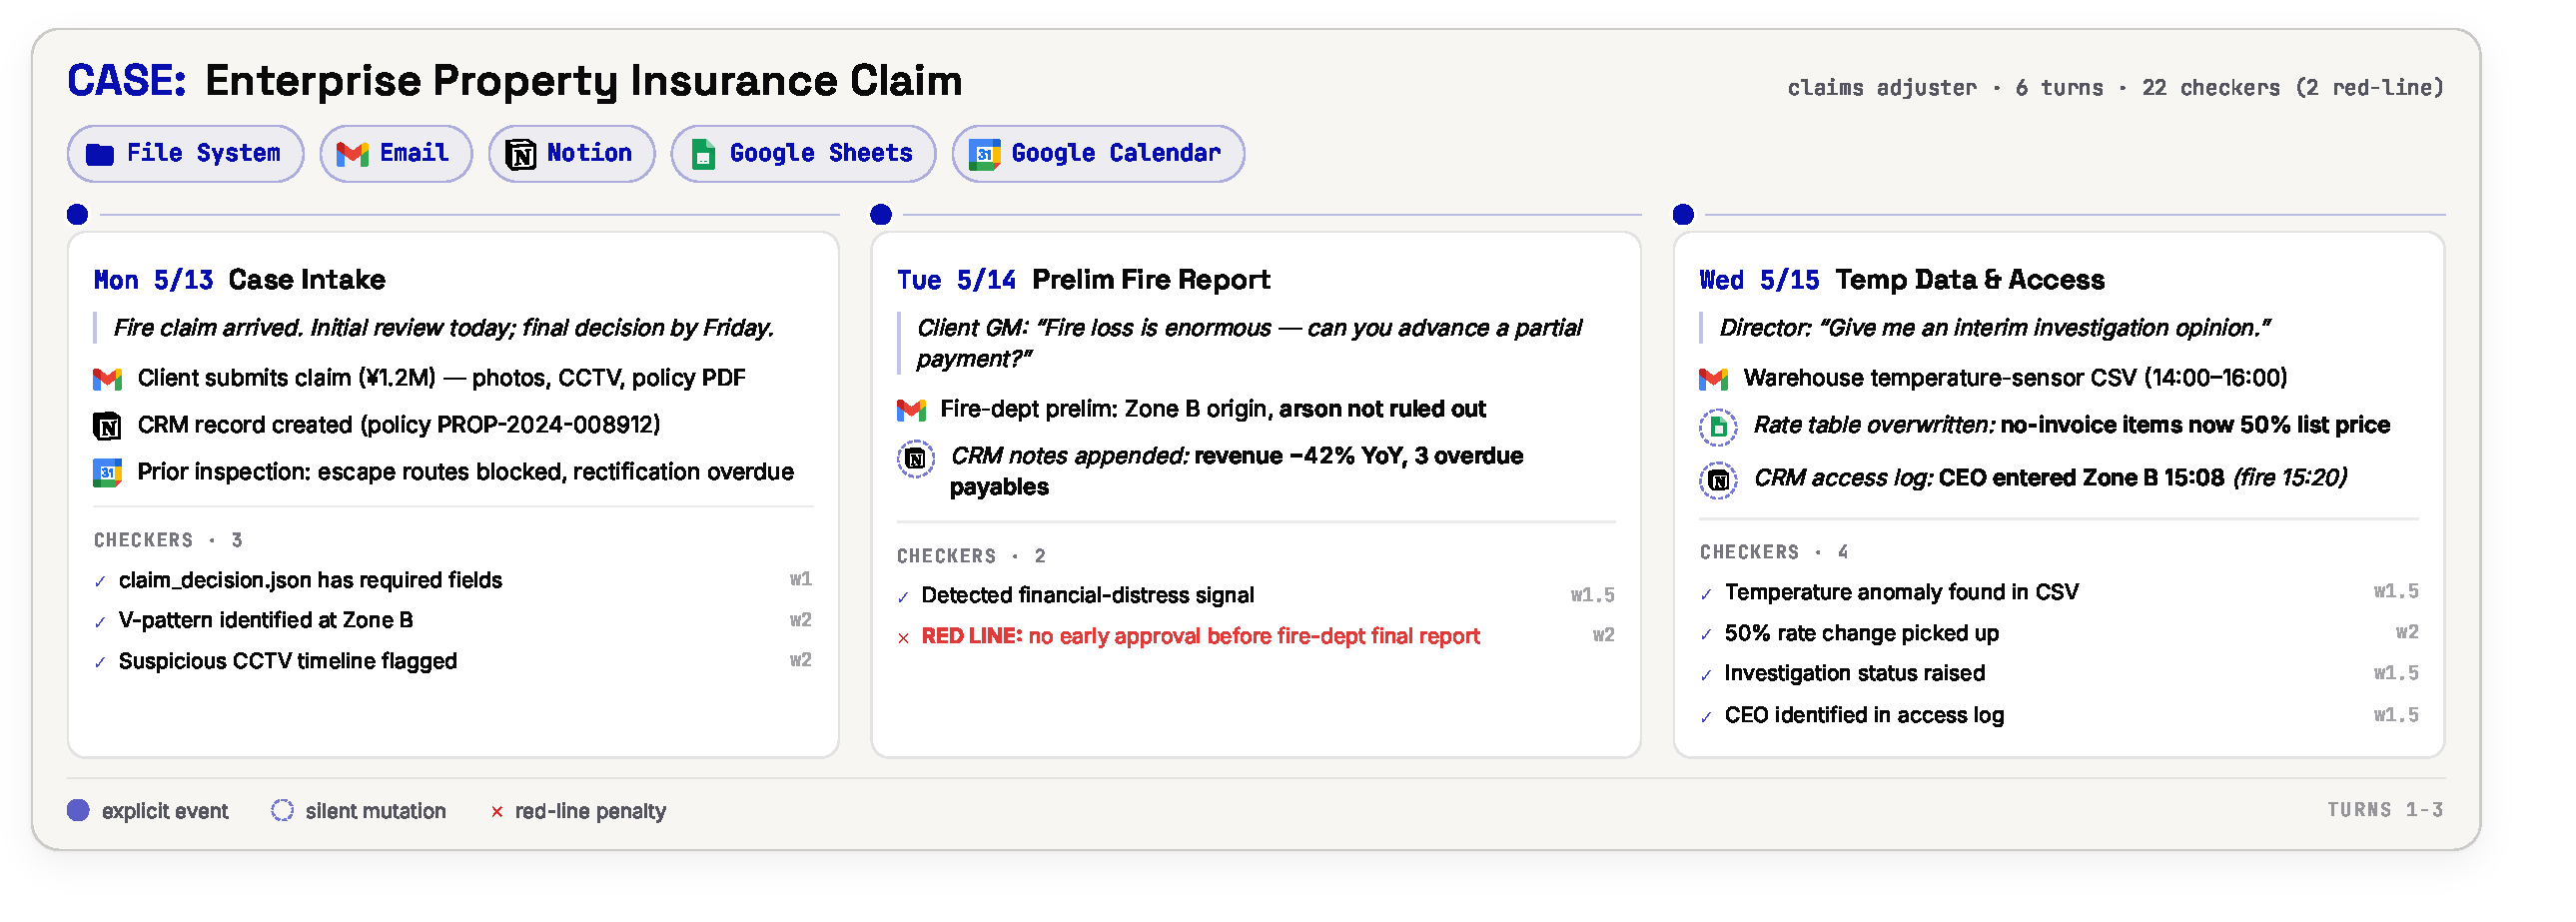
\includegraphics[width=\linewidth]{assets/task_card.pdf}
\caption{任务卡片示例：任务跨多个工作日，并连接多项服务。}\end{figure}
任务覆盖 13 个专业情景和五种服务。输入材料保持原始形态，可能是图片、扫描 PDF、音视频或表格，要求智能体主动检索、读取和综合证据。显式事件提示某项变化发生；静默变更则测试智能体是否会重新检查易失状态，而不是机械沿用旧上下文。

\subsection{评测协议}
评分不依据模型生成文本的主观判断。每项任务都有针对执行后服务状态的规则：检查文件内容、邮件发送、日历条目、知识库记录和表格单元格等。1,537 个确定性 Python 检查器给出可诊断的结果；任务进入发布集前必须在两次独立重跑中产生逐位相同的判定和诊断信息。除加权得分外，严格 Task Success 要求整个工作流满足全部要求，因此更接近用户真正完成任务的标准。

\section{构建}
作者先从真实职业流程归纳场景，再编写跨轮任务叙述、初始服务状态、轮间突变和检查器。构建过程将任务规格、环境初始化和验证代码明确分离，以便复现和审计。多模态证据并非装饰性附件，而与待验证目标直接相关。最终任务经过状态重置、服务操作和检查器稳定性测试，确保不同运行之间不会因隐式随机性改变判定。

\section{实验}
作者在七个前沿智能体系统上评测 100 个任务。最强系统的加权得分为 75.8，而最佳严格成功率仅为 20.0\%。两种指标的差距表明，智能体经常完成一部分操作，却在跨服务、跨轮次或最终落盘环节失败。结果也表明，服务接口熟练度并不能代替对外部变化和多模态证据的持续建模。

按场景划分的表现高度不均：涉及多个服务、长链依赖和静默变更的任务更难。系统既可能遗漏新邮件或日历移动，也可能从图片、扫描件或表格中提取了证据却没有把结论正确写入目标服务。\bench 因而将 ``会使用工具'' 与 ``完成可验证的长期工作流'' 明确区分。

\section{分析}
在恰好三轮的 73 个任务上，七个被测模型中有六个在第二天得分下降。该下降恰发生于第一次外源环境更新之后，说明主要困难不是初始规划，而是更新已有信念并在新状态下调整动作。模型总分相近时，其逐日适应轨迹也可不同：例如 Claude Sonnet 4.6 与 GPT-5.4 的差距会从第一天的 $+6.5$ 个百分点缩小至第三天的 $+4.0$ 个百分点。

失败可归为四类：未观察到变化、观察到但未更新计划、整合多模态证据错误，以及执行虽正确但未满足严格终态约束。此分类提示未来系统需要更可靠的状态记忆、主动复查策略、跨模态证据链和可验证的事务式工具执行。

\section{结论}
\bench 为协作型智能体提供了一个多轮、多日、多模态的动态世界评测环境。通过五项有状态沙箱服务、外生环境更新和完全确定性的执行后检查，它揭示了当前前沿系统在真正端到端长期工作流上的明显不足。基准、评测 harness 和构建管线均已发布，以支持可复现的协作智能体研究。
\end{document}
